\documentclass[openany]{article}

%Standard Stefanos Packages
\usepackage[utf8]{inputenc}
\usepackage{dirtytalk}
\usepackage{amsmath}
\usepackage{mathtools}  
\mathtoolsset{showonlyrefs} 
\usepackage{graphicx}
\usepackage{mdframed}
\usepackage{lipsum}
\usepackage{cancel}
\usepackage{systeme}
\usepackage{pgfplots}
\usepackage{textcomp}
\usepackage{geometry}
\usetikzlibrary{arrows}
\geometry{a4paper}
\graphicspath{ {./res/} }
\usepackage{float}
\restylefloat{table}
\usepackage{subcaption}
\newcommand{\comment}[1]{%
	\text{\phantom{(#1)}} \tag{#1}
}
\title{\line(1,0){450}\\ ST3MVA - Multivariate Data Analysis \\ \large{Coursework 2}  \\\line(1,0){450} \\University of Reading, 2021-2022}
\usepackage{pgfplots}
\author{Stefanos Stefanou}
\newmdtheoremenv{note}{Note}
\pgfplotsset{compat=1.17}

%Extra Packages
\usepackage{tikz}
\usetikzlibrary{automata,positioning}

\usepackage{listings}
\usepackage{xcolor}

\definecolor{dkgreen}{rgb}{0,0.6,0}
\definecolor{gray}{rgb}{0.5,0.5,0.5}
\definecolor{mauve}{rgb}{0.58,0,0.82}

\lstdefinestyle{myScalastyle}{
	frame=tb,
	language=scala,
	aboveskip=3mm,
	belowskip=3mm,
	showstringspaces=false,
	columns=flexible,
	basicstyle={\small\ttfamily},
	numbers=none,
	numberstyle=\tiny\color{gray},
	keywordstyle=\color{blue},
	commentstyle=\color{dkgreen},
	stringstyle=\color{mauve},
	frame=single,
	breaklines=true,
	breakatwhitespace=true,
	tabsize=3,
}
\begin{document}
	\maketitle
	\pagebreak
	
	\section*{Question 1}
	\begin{lstlisting}[language=R]
library(dplyr)

data <- read.csv("Spectroscopy.csv")
data$animal<-recode(data$animal,P="Pig",T="Turkey",C="Cattle")
attach(data)

wavelengths <- data[,3:17]
pairs(wavelengths,
pch=20,
col=recode(
data$animal,
Pig="#bc5090",
Turkey="#ff6361",
Cattle="#ffa600"))
	\end{lstlisting}
	%Spectroscopy-pairs
	
	\begin{figure}[H]
		\begin{subfigure}{\textwidth}
			\centering
			\includegraphics[scale=0.3]{res/Spectroscopy-pairs}
		\end{subfigure}
		
		\begin{subfigure}{\textwidth}
			\centering
			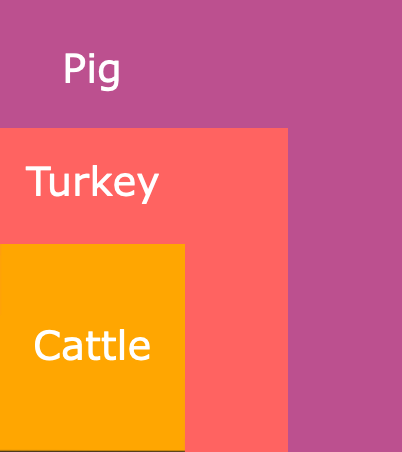
\includegraphics[scale=0.3]{res/Color-Map}
		\end{subfigure}
	\end{figure}
	\begin{itemize}
		\item WL8 Seems promising in separating Pig from Turkey and Cattle
		\item WL10 Seems promising in separating Turkey from Pig and Cattle
	\end{itemize}
	\pagebreak
	\begin{thebibliography}{1}	
		\bibitem{free-speech-us}
		\textit{En.wikipedia.org. 2021. United States Free Speech Exceptions. [online] Available at: <https://en.wikipedia.org/wiki/United\_States\_free\_speech\_exceptions> [Accessed 10 January 2021].}
		
	\end{thebibliography}
\end{document}